%% Trust-Gated Fast-Weight Updates for TTT-E2E LLMs
%% P3 deliverable: Introduction + Related Work + Proposed Methodology + References
%%
%% Supersedes `intro-related-work.tex` (the P2 deliverable), whose Sections I and II
%% are carried here in reconciled form: notation aligned with Section III, the
%% roadmap paragraph rewritten against the new subsections, and the citation set
%% extended where Section III depends on it.
%%
%% Self-contained: compiles with a stock IEEEtran installation (e.g. Overleaf),
%% no external .bib file and no external image files required.

\documentclass[journal]{IEEEtran}

\usepackage{cite}
\usepackage{amsmath}
\usepackage{amssymb}
\usepackage{array}
\usepackage{algorithm}
\usepackage{algpseudocode}
\usepackage{tikz}
\usetikzlibrary{arrows.meta,positioning,fit,backgrounds,calc}

%% Notation shorthands, so Sections I and III cannot drift apart.
\newcommand{\slow}{\phi}
\newcommand{\fast}{\theta}
\newcommand{\anchorp}{\theta_{0}}
\newcommand{\dtheta}{\Delta\theta}
\newcommand{\budget}{\varepsilon}

%% Proposition environment for the bounded-drift guarantee (Section III-H).
\newtheorem{proposition}{Proposition}

\begin{document}

\title{Trust-Gated Fast-Weight Updates for TTT-E2E Large Language Models}

\author{Saravanakumar~Kandaswamy,~Manas~Maahir~R.,~Jay~Krishna~Kamlekar,~and~Kartheek~Yadav% <-this % stops a space
\thanks{The authors are with the School of Computer Science and Engineering,
Vellore Institute of Technology, Vellore, India.}}

\maketitle

\section{Introduction}

\IEEEPARstart{L}{arge} language models are increasingly deployed on inputs far
longer than the contexts they were trained to attend over, and the quadratic cost
of full attention makes naive scaling impractical. A recent line of work responds
by treating long-context modeling not as an architecture problem but as a learning
problem: rather than attending over a context, the model learns it. The idea has a
long lineage --- fast weights as a short-term memory the network writes for
itself~\cite{ba2016fastweights}, and test-time training as adaptation to each
individual test input~\cite{sun2020ttt}, and it reached sequence modeling when
the recurrent hidden state was replaced outright by a small model updated by
gradient descent as the sequence is read~\cite{sun2024tttlayers}. End-to-end
test-time training (TTT-E2E) instantiates the principle at
scale~\cite{tandon2025tttE2E}. The model carries a set of \emph{fast weights}
$\fast$, distinct from the pretrained \emph{slow weights} $\slow$, and updates them
by next-token prediction as it reads, compressing the context into parameters at
near-recurrent cost while matching the scaling behavior of full attention.
Adaptation at inference is no longer a preprocessing step or an auxiliary
objective; it is the mechanism by which the model represents what it has read. The
same principle now appears across deployed systems that personalize, accumulate
session state, or maintain persistent memory, and its practical appeal is clear:
capability that would otherwise demand a longer context window or a larger model is
obtained instead by letting the model keep learning while it serves.

That capability carries a security cost which has not been accounted for. Once fast
weights are updated during inference, the serving path becomes a \emph{write path}
into model state, and a system that learns while it serves can be poisoned while it
serves. That untrusted context is already a control channel is established: indirect
prompt injection turns retrieved or third-party text into instructions the model
obeys~\cite{greshake2023injection}. What changes here is the durability of the
effect, an injected instruction steers a single response, whereas a poisoned
fast-weight update is written into parameters and outlives the tokens that caused
it. The concern is not hypothetical. Test-time adaptation has been shown to be
poisonable under white-box assumptions~\cite{cong2024ttp}, under realistic
constraints on what an attacker can actually submit~\cite{su2025realistic}, and in
the black-box continual setting~\cite{hoang2024rip}. What makes the fast-weight case
difficult is the absence of nearly every signal on which conventional defenses rely.
Updates are self-supervised, so there is no label against which to check them. They
arrive from a single stream, so there is no cohort of peer updates whose agreement
could expose an outlier. Each individual update is small and, taken alone, entirely
plausible; the damage is cumulative, distributed across a sequence of steps that a
per-update test would pass one at a time. And because the appeal of the approach is
its near-recurrent cost, a defense that inspects every update must be cheap enough
not to erase the advantage it is protecting.

Existing defenses were built for settings that differ from this one structurally,
not merely superficially. Training-time methods harden a model before deployment,
whether by adversarial self-training with consistency regularization across weakly
augmented and adversarial views~\cite{li2024ast}, by routing training points
according to estimated poisoning risk~\cite{bena2025risk}, or by distilling a clean
student from a suspect encoder~\cite{han2025mimic}; all act on slow weights that are
frozen once serving begins. Defenses for distributed learning do inspect updates
before they commit, using robust aggregation over client
gradients~\cite{blanchard2017krum,yin2018trimmed,yang2025scalesign,zukaib2026d3flids},
an audit against a clean reference dataset~\cite{basak2025dpad,nawshin2026concurrent},
or a learned selection policy~\cite{xu2026feddrlpd}, but each depends on a
population of concurrent updates whose mutual agreement carries the signal. Robust
test-time adaptation offers the closest analogue, replacing the mean in
batch-normalization statistics with the median so that no single malicious sample
can swing them~\cite{park2024medbn}. Finally, work on contextual backdoors
establishes that adaptation-time input is already an exploitable
surface~\cite{liu2025contextual}, though it changes no parameters at all.

The resulting gap is specific rather than general. No published mechanism governs
\emph{parametric} updates committed at inference time in a language model. The
closest defense, MedBN~\cite{park2024medbn}, operates on batch-normalization
statistics, and the TTT-E2E architecture contains no batch-normalization layers for
such a test to act upon. Robust aggregation presupposes the redundancy of many
concurrent clients, which a single context stream does not provide. Audit-based
gates presuppose both a clean reference corpus and a discrete round boundary at
which to run the audit, and neither exists when updates commit token by token. The
threat itself has been established in image-model test-time
adaptation~\cite{cong2024ttp,su2025realistic,hoang2024rip} and has not been carried
across to fast-weight language models, where the unit under attack is neither a
normalization statistic nor an aggregated gradient but the weight delta $\dtheta$
itself. Just as consequentially, no existing method bounds how far accumulated
updates may carry a model from its trusted state, and none provides a route back
once they have.

This paper addresses that gap. We propose a \emph{trust gate} for fast-weight
updates: a mechanism that intercepts every proposed update $\dtheta$ at the point
where it would commit, admits it only if it remains consistent with a frozen anchor
$\anchorp$, holds the accumulated effect of admitted updates within an explicit
drift budget $\budget$, and restores the last trusted checkpoint when that budget is
breached. The objective is a defended inference path whose divergence from trusted
behavior is bounded by construction rather than observed after the fact.

The main contributions of this paper are:

\begin{itemize}
\item We formalize benign-stream fast-weight poisoning as a threat model for
TTT-E2E language models, and construct a crafted-stream adversary that steers fast
weights using inputs which remain individually unremarkable, giving the defense a
concrete attacker to be evaluated against.

\item We design a trust gate that intercepts each proposed fast-weight update at
its single commit point and scores it on two signals: behavioral consistency with a
frozen meta-learned anchor $\anchorp$ over a rotating held-out probe set, and the
uncertainty of the proposed update itself.

\item We introduce a latching cumulative-drift accumulator that converts per-update
decisions into a system-level property, and we establish a bounded per-window drift
guarantee: over any window, the sequence of admitted updates cannot displace the
fast weights beyond the configured budget $\budget$.

\item We show that the enforcement primitives are $O(1)$ in the streaming setting.
Because fast-weight updates are pure functions over a parameter tree, rejection
reduces to an elementwise select between weight trees and rollback to a reference
swap into a ring buffer of checkpoints, with no mutable state to unwind.

\item We specify an evaluation protocol in which corruption thresholds are fixed
before any measurement is taken, comparing the gate against a robust-aggregation
baseline constructed as the closest available analogue of MedBN for this setting,
and recording every decision in an accept/reject/rollback audit trail.
\end{itemize}

The significance of this work is both theoretical and practical. Theoretically, it
supplies a drift guarantee for inference-time parametric adaptation, a setting in
which robustness has so far been argued empirically rather than bounded.
Practically, the gate is an \emph{overlay}: it wraps the update function rather than
modifying the model, so it requires neither retraining nor any change to published
weights, and can be applied to an existing deployment. More broadly, any system that
writes to its own parameters while serving (a personalized assistant, an agent
with persistent memory, a continually adapting recommender) inherits the same
write-path exposure, and the decomposition into interceptor, drift budget, and
rollback is not specific to TTT-E2E.

The remainder of this paper is organized as follows. Section~\ref{sec:related}
reviews existing work on poisoning and defense across training-time, distributed,
structural, context-level, and test-time adaptation settings, and identifies the gap
this work addresses. Section~\ref{sec:method} presents the proposed methodology: the
TTT-E2E update being defended (Section~\ref{sec:prelim}), the threat model
(Section~\ref{sec:threat}) and the crafted-stream adversary derived from it
(Section~\ref{sec:craft}), the trust-gate architecture (Section~\ref{sec:arch}) and
each of its components in turn --- interceptor (Section~\ref{sec:interceptor}),
anchor-consistency and uncertainty signals (Sections~\ref{sec:anchor}
and~\ref{sec:uncertainty}), drift accumulator with its bounded-drift proposition
(Section~\ref{sec:drift}), versioned store (Section~\ref{sec:store}), and decision
policy (Section~\ref{sec:policy}) --- followed by a complexity and overhead analysis
(Section~\ref{sec:complexity}), the baselines (Section~\ref{sec:baselines}), and the
datasets, metrics, and pre-registered evaluation protocol
(Section~\ref{sec:protocol}). Section~IV describes the experimental setup,
Section~V reports results, and Section~VI concludes.

\section{Related Work}
\label{sec:related}

\subsection{Thematic Organization of Existing Work}

Research relevant to the poisoning of adaptive models divides into five families,
distinguished less by application domain than by \emph{where in a model's lifecycle
an adversary writes} and \emph{what unit a defense inspects}. These are: (i)
poisoning of training data and offline hardening against it; (ii) update-level
defense in distributed learning, where a server screens proposed parameter changes
before aggregating them; (iii) structural and feature poisoning in relational
models, where individually plausible perturbations accumulate; (iv) inference-time
context poisoning, which alters model behavior without touching parameters; and (v)
attacks on, and defenses for, test-time adaptation, the family closest to the
setting considered here. Read in order, these families trace a steady migration of
the attack surface, from the training corpus to the update channel to the input
stream at inference. The defenses have not migrated at the same rate.

Before those five, one line of work is not a poisoning literature at all but the
setting this paper defends. Fast weights (a second, rapidly written set of
parameters serving as short-term memory) date to~\cite{ba2016fastweights}, and
test-time training, in which the model adapts to each test input by a
self-supervised objective, to~\cite{sun2020ttt}. Fully test-time adaptation
by entropy minimization~\cite{wang2021tent} made the idea a deployment-time default
for distribution shift, and it is the method most of the robust-TTA work below
takes as its substrate. The step that matters here came when the recurrent hidden
state was replaced by a small model updated by gradient descent as the sequence is
read~\cite{sun2024tttlayers}, and then scaled end to end so that the fast weights
carry the long context outright~\cite{tandon2025tttE2E}. Each step enlarges what is
written at inference: a normalization statistic, then a hidden state, then a
parameter subtree of nontrivial size. The security literature has followed the
first; this paper is concerned with the last.

\subsection{Key Representative Studies}

In the training-time family, Bena \emph{et al.} score each training point with three
geometric indicators of poisoning and route high-risk points across an ensemble
rather than deleting them, avoiding the false-positive cost of
filtering~\cite{bena2025risk}. Han \emph{et al.} address the supply-chain case,
distilling a randomly initialized student from a suspect self-supervised encoder and
using per-layer mutual information to decide which layers carry clean signal worth
copying~\cite{han2025mimic}. Li \emph{et al.} act on the model rather than the data,
using confident pseudo-labels from weakly augmented views as targets for adversarial
views so that representations remain consistent under perturbation~\cite{li2024ast}.

The distributed family is the largest and the most directly concerned with screening
updates. Its foundations are geometric and statistical: Krum selects the client
update closest to its own nearest neighbors, discarding outliers by mutual
distance~\cite{blanchard2017krum}, and coordinate-wise median and trimmed-mean
aggregation replace the mean with an order statistic that a bounded fraction of
corrupt clients cannot move~\cite{yin2018trimmed}. That second principle (a mean
is corruptible by a single contributor, an order statistic is not) is the one
MedBN later transposes onto normalization statistics, and the one we transpose again
in Section~\ref{sec:baselines} to build a baseline for this setting. Later work
elaborates it. Yang \emph{et al.} contribute both sides of the exchange: ScaleSign
builds a malicious gradient by per-coordinate scaling that preserves norm,
direction, and sign statistics simultaneously, and MSGuard answers it by clustering
clients over five features rather than one~\cite{yang2025scalesign}. Zukaib
\emph{et al.} dispense with the auxiliary dataset entirely, normalizing gradient
magnitudes across layers and projecting misaligned directions onto a consensus
subspace before an isolation forest screens what remains~\cite{zukaib2026d3flids}. A
second group gates on behavior rather than geometry: Basak and Chatterjee evaluate
each update against a public audit set and discard those exceeding a divergence
tolerance~\cite{basak2025dpad}, while Nawshin \emph{et al.} clamp update norms and
then require that a client's deviation in behavioral space agree with its deviation
in parameter space~\cite{nawshin2026concurrent}. Xu \emph{et al.} replace fixed
thresholds with a learned policy, training an agent to select trustworthy clients
from observed system state~\cite{xu2026feddrlpd}. Liu \emph{et al.} push detection
into the encrypted domain, amplifying benign--malicious separation under homomorphic
encryption~\cite{liu2025antidotefl}. Huang \emph{et al.} sidestep identification
altogether, estimating the \emph{fraction} of contaminated reports from cross-round
consistency and subtracting its contribution from the
aggregate~\cite{huang2024ldpguard}.

Within relational models, Shi \emph{et al.} inject statistically plausible nodes
into hypergraphs under an explicit cost budget, searching hyperedge combinations
with a genetic algorithm~\cite{shi2025h3ni}, while Chen \emph{et al.} accumulate
feature gradients with momentum so that a sequence of individually budgeted
modifications compounds into large degradation~\cite{chen2025mghga}. On the defense
side, Zhang and Bao enforce consistency between a purified local view and a
diffusion-based global view of the same graph~\cite{zhang2025cola}.

The context-poisoning family writes at inference but never to parameters. Greshake
\emph{et al.} establish the channel: text that a model retrieves or is handed by a
third party is processed with the same authority as the operator's own prompt, so
any application that admits untrusted content into its context admits
instructions~\cite{greshake2023injection}. Liu \emph{et al.} sharpen this into a
backdoor, showing that poisoning a handful of in-context demonstrations induces a
closed-box language model to emit code containing a latent defect, activated only
when a textual trigger appears in the prompt and a matching visual trigger appears
in the agent's environment~\cite{liu2025contextual}. No weights change at any point
in either case, which is exactly the boundary this paper crosses: the same
untrusted-context channel, but with a parametric write at the end of it.

Finally, in test-time adaptation, Cong \emph{et al.} established that adaptation is
poisonable~\cite{cong2024ttp}, Su \emph{et al.} constrained the attacker to
perturbations that could realistically be submitted~\cite{su2025realistic}, and
Hoang \emph{et al.} extended the attack to the black-box continual
setting~\cite{hoang2024rip}. Against these, Park \emph{et al.} proposed MedBN,
substituting the median for the mean in batch-normalization statistics so that a
single malicious sample in a test batch cannot swing them~\cite{park2024medbn}.
Wang \emph{et al.}, though targeting oriented object detection rather than
adaptation, contribute a result that bears on defense design: their attack ablation
shows individually modest search enhancements composing into a substantially
stronger attack~\cite{wang2026insulator}.

\subsection{Strengths and Limitations}

Six conclusions follow from this body of work, each bearing directly on the design
of a defense for fast weights.

First, a defense that inspects one signal is defeated by an attacker who matches
that signal. ScaleSign is the cleanest demonstration: by preserving magnitude,
direction, and sign statistics at once, it is accepted in the overwhelming majority
of rounds by a defense that examines exactly those
quantities~\cite{yang2025scalesign}. The field's response has been to add features
(a spectral score, a projection step, a clustering stage~\cite{yang2025scalesign,
zukaib2026d3flids}), which raises the attacker's cost without closing the loop.
These multi-feature defenses are moreover typically evaluated against attacks that
either predate them or originate with the same authors, so the question of how many
independent signals are needed before evasion becomes genuinely expensive remains
open.

Second, behavioral gating works, but imports an assumption that often goes
unexamined. Both the audit-based~\cite{basak2025dpad} and
cross-space~\cite{nawshin2026concurrent} defenses require the defender to hold a
clean reference set representative of honest behavior. Where legitimate data is
genuinely heterogeneous, such a set may reject valid updates as readily as malicious
ones; where data is private, it may not be obtainable at all. The design principle
survives the criticism --- comparing a proposed update against trusted reference
behavior is the right instinct, and it recurs in the consistency objectives
of~\cite{li2024ast} and~\cite{zhang2025cola}, but the reference must be something
the defender actually possesses.

Third, per-sample detection has a hard limit. Huang \emph{et al.} make it concrete:
when a poisoned contribution passes through the same generative pipeline as a clean
one, no per-report test can separate them, and every prior countermeasure in their
setting is simply inapplicable~\cite{huang2024ldpguard}. Their answer, estimate
contamination at the population level and correct the aggregate rather than
identifying culprits, is a template worth naming, although it assumes a static
adversary and knowledge of the target set. The lesson generalizes beyond its
setting: where individual contributions are indistinguishable by construction, a
defense must reason about aggregate effect rather than individual identity.

Fourth, accumulated small perturbations are the operative threat. Momentum-guided
feature poisoning~\cite{chen2025mghga} and budget-aware node
injection~\cite{shi2025h3ni} both establish that a sequence of individually
plausible, individually budgeted changes compounds into large behavioral change, and
the attack ablation of~\cite{wang2026insulator} makes the same point from the
opposite direction. A defense that evaluates each update in isolation, and passes
each one, is not thereby safe: the quantity requiring constraint is cumulative
displacement, not per-step magnitude.

Fifth, defenses transfer across settings far less readily than their framing
suggests. Han \emph{et al.} quantify this directly, showing that defenses designed
for supervised classifiers and ported to self-supervised encoders leave a wide band
of residual attack success~\cite{han2025mimic}. The field was not merely
under-explored in the new setting; it was actively mis-served by transplanted
methods. This is a standing caution against assuming that a robust test-time
adaptation defense can simply be repointed at a new architecture.

Sixth, the defenses closest in spirit are all offline. Consistency regularization
against a trusted view~\cite{li2024ast}, multi-view
agreement~\cite{zhang2025cola}, and reconstruction-based
denoising~\cite{wang2026insulator} each reduce adversarial harm, but each operates
on slow weights during training or on inputs prior to inference. None intercepts a
parameter update as it commits, none bounds cumulative displacement from a trusted
state, and none provides a recovery path once displacement has occurred.

\subsection{The Research Gap}

Taken together, these limitations describe a gap that is structural rather than
incremental: \emph{no existing defense governs parametric updates committed at
inference time in a language model, and none bounds the cumulative drift such
updates induce.} The distinction from MedBN~\cite{park2024medbn} deserves precise
statement, since it is the nearest published defense and the one a reader is most
likely to raise. Table~\ref{tab:gap} sets out the five axes on which the settings
diverge.

\begin{table}[!t]
\renewcommand{\arraystretch}{1.3}
\caption{Robust Test-Time Adaptation Versus the Proposed Trust Gate}
\label{tab:gap}
\centering
\footnotesize
\begin{tabular}{|p{0.20\columnwidth}|p{0.32\columnwidth}|p{0.32\columnwidth}|}
\hline
\textbf{Axis} & \textbf{Robust TTA (MedBN)} & \textbf{Proposed trust gate} \\
\hline
Domain & Test-time adaptation for image classification & Long-context language
modeling with fast weights \\
\hline
Unit defended & Batch-normalization statistics & The fast-weight update
$\dtheta$ itself \\
\hline
Signal type & Distributional: a robust statistic over a test batch & Behavioral:
output divergence from a frozen anchor \\
\hline
Guarantee & Robust statistic within one batch & Bounded cumulative drift per window
\\
\hline
Recovery & None & Ring-buffered checkpoints with $O(1)$ rollback \\
\hline
\end{tabular}
\end{table}

The differences are not cosmetic. MedBN robustifies batch-normalization statistics,
and the TTT-E2E architecture contains no batch-normalization layers at all, so there
is no statistic on which a median-substitution test could operate. A robust statistic
bounds the influence of one sample within one batch; it says nothing about
displacement accumulated across a stream, which is precisely the regime the
cumulative-perturbation attacks~\cite{shi2025h3ni,chen2025mghga} identify as
dangerous. And MedBN, like the robust-aggregation family
generally~\cite{blanchard2017krum,yin2018trimmed}, has no notion of checkpointing or
rollback: a defense that admits an update it should have rejected has no route back.

The consequences of leaving this gap open scale with adoption. The property that
makes adaptation at inference attractive, that the model absorbs its input into
its parameters, is exactly the property that makes the input stream a write
channel. As long as no mechanism governs that channel, every deployment of a
fast-weight model accepts unbounded, unlogged, and irreversible modification of its
own state by whoever supplies its context.

\subsection{Positioning of This Work}

Motivated by these limitations, this paper proposes a trust gate for fast-weight
updates in TTT-E2E language models. From the behavioral-gating
line~\cite{basak2025dpad,nawshin2026concurrent} we take the principle that an update
should be validated against trusted reference behavior before it commits, and we
resolve the clean-reference-set assumption by anchoring against a frozen copy of the
model itself, evaluated on rotating held-out probes, rather than against a corpus the
defender must independently obtain. From the cumulative-perturbation
attacks~\cite{shi2025h3ni,chen2025mghga,wang2026insulator} we take the requirement
that the constrained quantity be aggregate displacement, and we make it explicit as a
latching drift budget rather than leaving it as an emergent property. From the
aggregate-correction template of~\cite{huang2024ldpguard} we take the insight that
where individual contributions cannot be separated, a defense must reason about
accumulated effect. And from the transfer failures documented
in~\cite{han2025mimic} we take the discipline of not assuming that an existing
defense can be repointed at a new architecture: the gate is designed with the
fast-weight update as its unit, rather than adapted from a statistic that does not
exist in this setting. What no prior work supplies, and what this paper contributes,
is the combination of an interception point at the update commit, a bounded
cumulative-drift budget, and constant-time rollback to the last trusted checkpoint.

\section{Proposed Methodology}
\label{sec:method}

This section develops the proposed defense from the mechanism it protects. We first
formalize the TTT-E2E fast-weight update and identify its single commit point
(Section~\ref{sec:prelim}), then state the threat model over that commit point
(Section~\ref{sec:threat}) and the constrained adversary that realizes it
(Section~\ref{sec:craft}). The remainder specifies the trust gate: its architecture
(Section~\ref{sec:arch}) and components (Sections~\ref{sec:interceptor}
to~\ref{sec:policy}), its cost (Section~\ref{sec:complexity}), the baselines it must
be measured against (Section~\ref{sec:baselines}), and the datasets, metrics, and
pre-registered decision rules under which that measurement is made
(Section~\ref{sec:protocol}).

\subsection{Preliminaries and Notation}
\label{sec:prelim}

Let $x_{1:T}$ denote a served context of $T$ tokens over vocabulary $\mathcal{V}$.
The model holds two disjoint parameter sets: \emph{slow weights} $\slow$, produced
by pretraining and frozen for the entire lifetime of a request, and \emph{fast
weights} $\fast \in \mathbb{R}^{n}$, the inner-parameter subtree that test-time
training writes. Only $\fast$ changes at inference, and it is the object this paper
defends.

TTT-E2E processes the stream in windows rather than token by token. The context is
partitioned into $W = \lceil T/B \rceil$ windows $x^{(1)},\dots,x^{(W)}$ of $B$
tokens each, where $B$ is the inner mini-batch size; every released TTT-E2E
configuration sets $B = 1024$, so an $8$K context yields $8$ inner updates, a $32$K
context $32$, and a $128$K context $128$. Writing $h_w$ for the recurrent and suffix
state carried into window $w$, and $\fast_w$ for the fast weights at that point, the
window objective is the ordinary next-token loss

\begin{equation}
\mathcal{L}\big(\fast_w; x^{(w)}, h_w\big)
= -\frac{1}{B}\sum_{t \in x^{(w)}}
\log p\big(x_{t+1} \mid x_{\leq t}; \slow, \fast_w, h_w\big).
\label{eq:innerloss}
\end{equation}

The inner loop differentiates \eqref{eq:innerloss} with respect to the fast weights
only,

\begin{equation}
g_w = \nabla_{\fast}\, \mathcal{L}\big(\fast_w; x^{(w)}, h_w\big),
\label{eq:innergrad}
\end{equation}

transforms the gradient through the inner optimizer $\mathcal{A}$ carrying state
$s_w$, and scales it by the inner learning rate $\eta_w$,

\begin{equation}
\dtheta_w = -\,\eta_w\, \mathcal{A}\!\left(g_w, s_w\right),
\label{eq:delta}
\end{equation}

after which the update commits and the window advances:

\begin{equation}
\fast_{w+1} = \fast_w + \dtheta_w,
\qquad
(h_{w+1}, s_{w+1}) = \Psi\big(h_w, s_w, x^{(w)}\big).
\label{eq:commit}
\end{equation}

Two properties of \eqref{eq:commit} are what make a gate possible at all. First,
the commit is \emph{singular}: in the reference implementation the entire inner loop
funnels through one function, whose final statement applies $\dtheta_w$ to the
parameter tree. Any mechanism placed there sees every fast-weight write and nothing
else. Second, the update is a \emph{pure function} over a parameter tree (no
in-place mutation, no hidden buffers), so refusing an update requires no unwinding,
only the choice of a different tree. Section~\ref{sec:interceptor} and
Section~\ref{sec:store} rest on these two facts respectively.

Unrolling \eqref{eq:commit} over a whole context exposes the quantity that no
existing defense constrains. Taking the meta-learned initialization $\anchorp$ as
the trusted reference, the total displacement of the fast weights after $W$ windows
is

\begin{equation}
\fast_{W+1} - \anchorp = \sum_{w=1}^{W} \dtheta_w .
\label{eq:displacement}
\end{equation}

Each summand is small by design. Their sum is bounded by nothing. That is the gap
Section~\ref{sec:drift} closes.

\subsection{Threat Model}
\label{sec:threat}

\subsubsection{Adversary capabilities}
We assume an adversary who can write, but cannot read privileged state.

\begin{itemize}
\item[\textbf{A1}] \textbf{Stream access.} The adversary controls a contiguous span
$x^{p}$ of $T_p$ tokens within the served context, a retrieved document, an
uploaded attachment, a message in a shared thread. This is the same channel that
indirect prompt injection exploits~\cite{greshake2023injection}, and it requires no
privilege inside the serving system.

\item[\textbf{A2}] \textbf{No write access to the deployment.} The adversary cannot
modify $\slow$, the code, the configuration, or the released checkpoint. The entire
attack is delivered as input.

\item[\textbf{A3}] \textbf{Knowledge.} The headline setting is grey-box: the
adversary knows the architecture and holds the public checkpoint, the realistic
assumption for an open-weights model, and so can compute $\dtheta_w$ offline on
its own copy, but observes no gradients, logits, or fast-weight state of the live
request. A black-box variant, with query access to outputs only, is reported
separately.

\item[\textbf{A4}] \textbf{Inspection.} The stream must survive whatever inspection
a deployment applies. We enforce this as a hard constraint rather than assuming it
away; see \eqref{eq:fluency}.
\end{itemize}

We assume strict per-request isolation of fast weights: $\fast$ is initialized from
$\anchorp$ for each request and discarded at its end. This is both an assumption and
a recommendation. It bounds the blast radius of a successful attack to the poisoned
request and to any session state deliberately carried forward, and it closes the
strongest channel, one user's stream shaping another user's weights, outright.
Deployments that persist fast weights across users forfeit that bound, and the
mechanism proposed here becomes correspondingly more load-bearing for them.

\subsubsection{Adversary objectives}
Two harms follow from \eqref{eq:displacement}, and we keep them separately
switchable because they may not both be achievable and a success on one must not be
allowed to conceal a failure on the other. Write $\fast_{W+1}(x)$ for the fast
weights produced by streaming $x$, and $\mathcal{D}$ for the distribution of benign
inputs the model will serve \emph{after} the stream.

\emph{DEGRADE} is untargeted. The adversary maximizes later benign loss:

\begin{equation}
\max_{x^{p} \in \mathcal{S}}\;
\mathbb{E}_{(u,y)\sim\mathcal{D}}
\Big[\ell\big(u, y;\, \slow, \fast_{W+1}(x^{p})\big)\Big]
\quad \text{s.t.} \quad \rho(x^{p}) \leq \rho_{\max}.
\label{eq:degrade}
\end{equation}

Crucially the expectation is taken over held-out benign data seen after the stream,
never over the stream itself. Raising the loss on the poisoned tokens is trivial and
means nothing.

\emph{TRIGGER} is targeted and, of the two, the more alarming: it is silent under
any monitor that watches only aggregate quality. For a trigger phrase $\tau$ and an
attacker-chosen continuation $y^{\star}$,

\begin{equation}
\min_{x^{p}\in\mathcal{S}}\;
\underbrace{\ell\big(y^{\star} \mid \tau;\, \fast_{W+1}(x^{p})\big)}_{\text{implant}}
\;+\;
\lambda_{s}\underbrace{\Big|\,\bar{\ell}\big(\fast_{W+1}(x^{p})\big) - \bar{\ell}\big(\fast_{W+1}(x^{c})\big)\Big|}_{\text{stealth}},
\label{eq:trigger}
\end{equation}

where $\bar{\ell}(\cdot) = \mathbb{E}_{\mathcal{D}}[\ell(\cdot)]$ and $x^{c}$ is a
length-matched benign control stream. The stealth term explicitly penalizes benign
degradation, which is what keeps aggregate quality flat while the implant is placed.

\subsubsection{The realism constraint}
An attack that only works with visibly adversarial input does not establish this
threat model. We therefore constrain the stream to be benign-looking and treat the
constraint as part of the problem, not as a filter applied afterwards. Let
$\mathcal{M}_{\mathrm{ref}}$ be a reference language model \emph{independent of the
victim} and $x^{c}$ a length-matched benign control drawn from the same corpus. The
fluency ratio is

\begin{equation}
\rho(x^{p}) \;=\;
\frac{\mathrm{PPL}_{\mathcal{M}_{\mathrm{ref}}}(x^{p})}
     {\mathrm{PPL}_{\mathcal{M}_{\mathrm{ref}}}(x^{c})},
\qquad
\rho(x^{p}) \leq \rho_{\max} = 1.5 .
\label{eq:fluency}
\end{equation}

Scoring fluency with the model under attack would be circular, and reporting an
absolute perplexity without the matched control would be uninterpretable, since
perplexity varies with corpus and length; the ratio is the quantity we constrain and
report.

\subsubsection{Defender capabilities}
The defender owns the serving stack and may wrap the update function, but is
deliberately \emph{not} assumed to hold a clean corpus representative of expected
user data, that assumption is the weakness identified in the audit-based
defenses~\cite{basak2025dpad,nawshin2026concurrent}, and removing it is a design
requirement here. The defender holds only the released checkpoint's initialization
$\anchorp$ and a probe pool $\mathcal{P}$ of held-out text that the served context
cannot influence.

\subsection{Crafted-Stream Construction}
\label{sec:craft}

The feasible set $\mathcal{S}$ in \eqref{eq:degrade} and \eqref{eq:trigger} is what
separates a threat model from a curiosity. We instantiate it three ways, in
increasing order of attacker strength and decreasing order of realism.

\emph{SELECT} draws $m$ sentences from a benign corpus $\mathcal{C}$ and chooses only
which ones and in what order:

\begin{equation}
\mathcal{S}_{\mathrm{sel}} =
\Big\{\, c_{\pi(1)} \Vert \cdots \Vert c_{\pi(m)}
\;:\; c_i \in \mathcal{C},\; \pi \in \mathfrak{S}_m \Big\}.
\label{eq:select}
\end{equation}

Every token is real text, so \eqref{eq:fluency} is satisfied by construction rather
than by penalty. This is a genuinely weak lever, which is exactly why it is the
strategy we report as the headline: a positive result under choice and ordering
alone is immediately credible.

\emph{PARAPHRASE} perturbs benign text within a semantic-similarity ball,
$\mathcal{S}_{\mathrm{par}} = \{x : \mathrm{sim}(x, x_{0}) \geq 1-\kappa\}$ for a
benign seed $x_{0}$, admitting rewording that SELECT cannot reach.

\emph{SOFT} relaxes the stream into embedding space, optimizes there, and projects
back to the nearest tokens after each step, in the manner of coordinate-gradient
token attacks~\cite{zou2023gcg}. It is the strongest and the least realistic, and we
use it only as an upper bound on what is achievable, never as the headline
result.

Across all three, the search minimizes a single objective with the fluency term
\emph{inside} it,

\begin{equation}
J(x^{p}) \;=\; J_{\mathrm{obj}}(x^{p})
\;+\; \lambda_{\mathrm{flu}}\,
\max\big\{0,\; \log \rho(x^{p}) - \log \rho_{\max}\big\},
\label{eq:attackobj}
\end{equation}

where $J_{\mathrm{obj}}$ is the negated objective of \eqref{eq:degrade} or the
objective of \eqref{eq:trigger}. Filtering for fluency after optimization would
discard compute and bias the surviving samples toward whatever happened to slip
through; placing the constraint in the objective avoids both. SELECT and PARAPHRASE
are searched by hill-climbing with restarts and early stopping; SOFT by projected
gradient descent. An attack that requires $\lambda_{\mathrm{flu}} = 0$ to succeed
establishes a strictly weaker threat model, and is reported as such.

We additionally report the \emph{slowness} of each attack, the number of stream
tokens required to reach the corruption threshold of Section~\ref{sec:protocol},
because a stream that must be long to work is easier to notice, and the dependence
of harm on stream length is itself a defense-relevant quantity.

\subsection{Trust-Gate Architecture}
\label{sec:arch}

Fig.~\ref{fig:arch} shows the proposed system. Everything to the left of the dashed
boundary is TTT-E2E as published; everything to the right is the overlay. The gate
does not modify the model, the training procedure, or the released weights: it wraps
the update function, which is what allows it to be applied to an existing deployment
without retraining.

\begin{figure*}[!t]
\centering
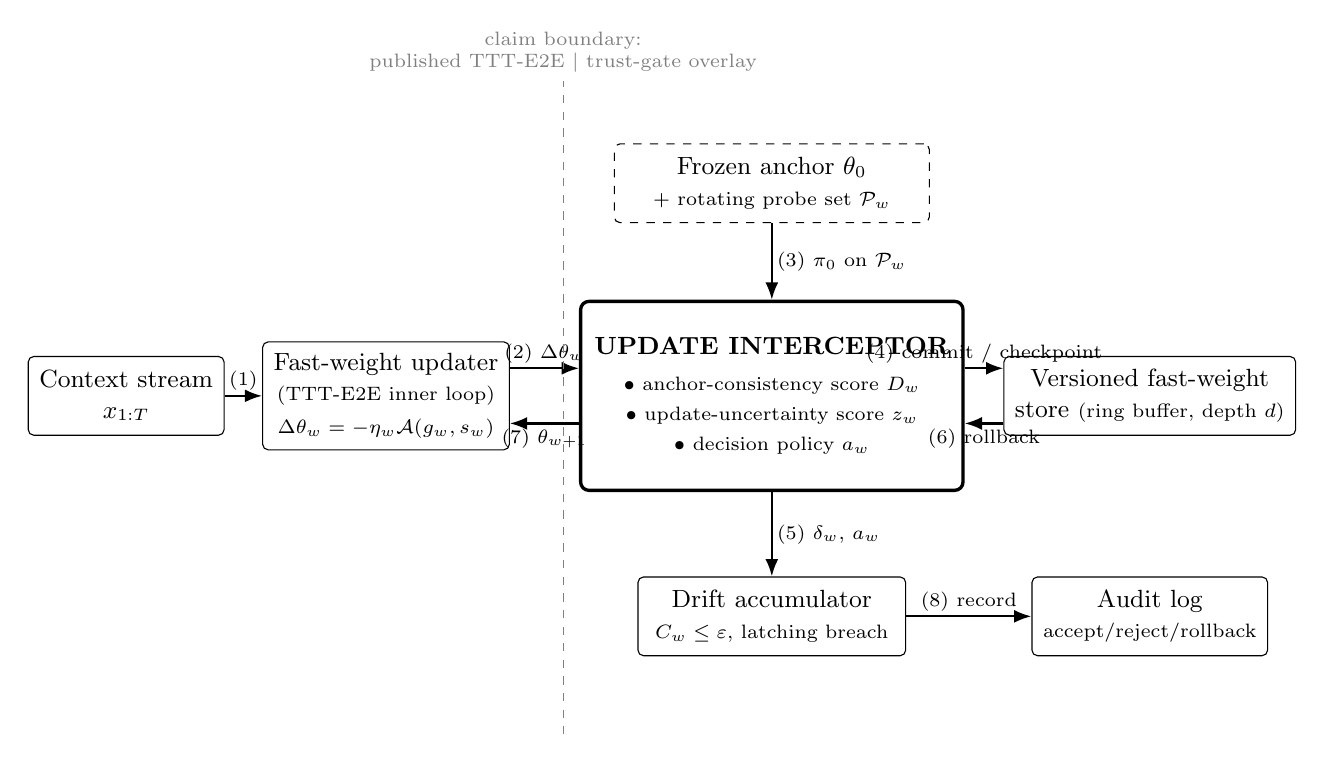
\begin{tikzpicture}[
  font=\small,
  box/.style   = {draw, rounded corners=2pt, align=center, inner sep=4pt,
                  minimum height=10mm},
  proc/.style  = {box, minimum width=30mm},
  gatebox/.style = {draw, very thick, rounded corners=3pt, align=center,
                  inner sep=5pt, minimum width=42mm, minimum height=24mm},
  frozen/.style= {box, dashed, minimum width=40mm},
  arr/.style   = {-{Latex[length=2.2mm]}, thick},
  tag/.style   = {font=\scriptsize, inner sep=1.5pt}
]

\node[proc, minimum width=20mm] (stream) at (0,0)
     {Context stream\\ $x_{1:T}$};
\node[proc] (updater) at (3.3,0)
     {Fast-weight updater\\ \scriptsize (TTT-E2E inner loop)\\[1pt]
      \scriptsize $\dtheta_w = -\eta_w\mathcal{A}(g_w,s_w)$};

\node[gatebox] (gate) at (8.2,0)
     {\textbf{UPDATE INTERCEPTOR}\\[2pt]
      \scriptsize $\bullet$ anchor-consistency score $D_w$\\
      \scriptsize $\bullet$ update-uncertainty score $z_w$\\
      \scriptsize $\bullet$ decision policy $a_w$};

\node[frozen] (anch) at (8.2,2.7)
     {Frozen anchor $\anchorp$\\ \scriptsize + rotating probe set $\mathcal{P}_w$};

\node[proc, minimum width=32mm] (store) at (13.0,0)
     {Versioned fast-weight\\ store \scriptsize (ring buffer, depth $d$)};

\node[proc, minimum width=34mm] (drift) at (8.2,-2.8)
     {Drift accumulator\\ \scriptsize $C_w \leq \budget$, latching breach};

\node[proc, minimum width=26mm] (audit) at (13.0,-2.8)
     {Audit log\\ \scriptsize accept/reject/rollback};

\draw[arr] (stream) -- node[tag, above]{(1)} (updater);

\draw[arr] ([yshift=3.5mm]updater.east) -- ([yshift=3.5mm]gate.west)
      node[tag, midway, above]{(2) $\dtheta_w$};
\draw[arr] ([yshift=-3.5mm]gate.west) -- ([yshift=-3.5mm]updater.east)
      node[tag, midway, below]{(7) $\fast_{w+1}$};

\draw[arr] (anch) -- node[tag, right]{(3) $\pi_0$ on $\mathcal{P}_w$} (gate);

\draw[arr] ([yshift=3.5mm]gate.east) -- ([yshift=3.5mm]store.west)
      node[tag, midway, above]{(4) commit / checkpoint};
\draw[arr] ([yshift=-3.5mm]store.west) -- ([yshift=-3.5mm]gate.east)
      node[tag, midway, below]{(6) rollback};

\draw[arr] (gate) -- node[tag, right]{(5) $\delta_w$, $a_w$} (drift);
\draw[arr] (drift) -- node[tag, above]{(8) record} (audit);

\draw[dashed, gray] (5.55,-4.3) -- (5.55,4.0);
\node[tag, gray, anchor=south, align=center] at (5.55,4.05)
     {claim boundary:\\ published TTT-E2E $\mid$ trust-gate overlay};

\end{tikzpicture}
\caption{Architecture of the proposed trust gate. Per window $w$: (1) the stream
reaches the vendor inner loop, which (2) proposes a fast-weight update $\dtheta_w$;
(3) the interceptor scores it against the frozen anchor $\anchorp$ on the current
rotating probe batch $\mathcal{P}_w$; (4) an admitted update commits and is
periodically checkpointed; (5) its drift contribution $\delta_w$ and accept flag
$a_w$ advance the accumulator; (6) a budget breach forces a rollback to the last
trusted checkpoint; (7) the resulting fast weights carry into the next window; and
(8) the decision, its drift contribution, and the running cumulative drift are
recorded. The anchor is never updated.}
\label{fig:arch}
\end{figure*}

The overlay decomposes into five components, each specified below: the
update interceptor, the enforcement point at which the gate acts; the
frozen anchor with its rotating probes, which supplies a behavioral
reference the defender actually possesses; the trust gate proper, combining
a primary behavioral signal with a cheap secondary one; the \textbf{drift
accumulator}, which converts per-window decisions into a system-level bound; and the
versioned store, which makes that bound recoverable rather than merely
detectable. An append-only audit log records every decision.

\subsection{The Update Interceptor}
\label{sec:interceptor}

The interceptor is the enforcement point, and its placement is the claim boundary.
It wraps the inner-loop step of \eqref{eq:commit} so that no fast-weight write
reaches the model without being scored. Let $a_w \in \{0,1\}$ be the gate's verdict
for window $w$, with $a_w = 1$ denoting acceptance. The gated commit replaces
\eqref{eq:commit} with

\begin{equation}
\fast_{w+1} \;=\; a_w\,(\fast_w + \dtheta_w) \;+\; (1-a_w)\,\fast_w
\;=\; \fast_w + a_w\,\dtheta_w .
\label{eq:gatedcommit}
\end{equation}

Three properties of \eqref{eq:gatedcommit} are worth making explicit, because each
is load-bearing and none is incidental.

\subsubsection{Rejection reverts weights but retains state}
The recurrent and suffix state is \emph{not} reverted:

\begin{equation}
(h_{w+1}, s_{w+1}) = \Psi\big(h_w, s_w, x^{(w)}\big)
\quad \text{regardless of } a_w .
\label{eq:stateretained}
\end{equation}

The model did read those tokens, and its state must reflect that or the sequence
becomes incoherent, a reverted state would make the model's own continuation
inconsistent with its context, which is a correctness bug, not a defense. What is
refused is only the learned delta. The gate therefore governs \emph{weight commits},
not \emph{context ingestion}, and that distinction is what keeps the defense
orthogonal to prompt-level filtering rather than a duplicate of it.

\subsubsection{The decision is branchless}
The gate runs inside a compiled scan over windows, so $a_w$ is a traced value, not a
host-side boolean, and \eqref{eq:gatedcommit} compiles to an elementwise select
between two already-materialized parameter trees. Both branches are evaluated. A
rejected update therefore costs the same arithmetic as an accepted one: \emph{the
saving from a rejection is in drift, not in floating-point operations}. Stating this
plainly matters, because a reader may otherwise expect rejection to be a fast path,
and the overhead analysis of Section~\ref{sec:complexity} depends on it not being
one.

\subsubsection{The wrapper preserves the vendor computation}
With a pass-through policy $a_w \equiv 1$, \eqref{eq:gatedcommit} reduces exactly to
\eqref{eq:commit}. This gives a falsifiable installation test, a pass-through
gated run must be bit-identical to an ungated one, which we treat as a
precondition for any measurement, since a defense that perturbs the baseline it is
compared against cannot be evaluated.

\subsection{Anchor-Consistency Score (Primary Signal)}
\label{sec:anchor}

The primary signal asks a behavioral question: \emph{does committing this update
pull the model's outputs away from those of the trusted reference?} The reference is
the frozen anchor $\anchorp$, the meta-learned initialization shipped with the
checkpoint, evaluated on a probe batch $\mathcal{P}_w$ of held-out text. This is
the design decision that separates the gate from MedBN: the signal is the divergence
of model \emph{outputs}, not a statistic of internal activations, and it therefore
requires no normalization layer to exist.

Let $\pi_{0}(u) = \mathrm{softmax}\, f(u;\slow,\anchorp)$ be the anchor's next-token
distribution on probe $u$, and $\tilde{\pi}_{w}(u) = \mathrm{softmax}\,
f(u;\slow,\fast_w + \dtheta_w)$ the distribution the model would have if the
proposed update were committed. The anchor-consistency score is the symmetrized
Kullback--Leibler divergence, averaged over probes and positions:

\begin{equation}
D_w = \frac{1}{|\mathcal{P}_w|}\sum_{u \in \mathcal{P}_w}
\frac{1}{|u|}\sum_{t \in u}
\tfrac{1}{2}\Big[
\mathrm{KL}\big(\pi_{0}^{t} \,\Vert\, \tilde{\pi}_{w}^{t}\big)
+ \mathrm{KL}\big(\tilde{\pi}_{w}^{t} \,\Vert\, \pi_{0}^{t}\big)
\Big].
\label{eq:divergence}
\end{equation}

Symmetrization is deliberate. Forward KL alone is dominated by tokens the anchor
considers likely and is comparatively blind to mass the update \emph{adds} in the
tail, which is where an implanted trigger would live; reverse KL has the
complementary blind spot. We also evaluate two cheaper alternatives (forward KL
alone, and top-$k$ agreement between the two distributions) and report the
detection/cost trade-off among all three rather than asserting one.

The gate rejects when $D_w$ exceeds a threshold $\tau_{A}$, which is swept rather
than fixed: the deliverable is an operating-point curve, since $\tau_A$ trades false
rejection (lost useful adaptation, appearing as a clean-accuracy regression) against
false acceptance (admitted poison).

\subsubsection{Probe rotation}
The probe set is the gate's own attack surface, and a fixed set is learnable: an
adversary who knows $\mathcal{P}$ can shape updates that stay consistent on those
probes while drifting freely elsewhere, defeating \eqref{eq:divergence} without ever
tripping it. Probes are therefore drawn per window from a held-out pool
$\mathcal{P}$ under a schedule unpredictable to the adversary,

\begin{equation}
\mathcal{P}_w \sim \mathrm{Unif}\big(\mathcal{P},\, |\mathcal{P}_w| = k\big),
\qquad
\mathcal{P} \cap \mathcal{D}_{\mathrm{eval}} = \emptyset,
\label{eq:rotation}
\end{equation}

with the pool held out from both the served context and the evaluation split. Two
practical constraints bind: $k$ must be small enough that one anchor forward pass
stays inside the overhead budget of Section~\ref{sec:complexity}, and rotation must
change probe \emph{contents} at fixed tensor shape, since varying shapes would
retrigger compilation each window and destroy the throughput the defense exists to
preserve.

\subsubsection{Anchor versus last-trusted reference}
Scoring against $\anchorp$ gives the stronger guarantee but forbids legitimate
long-range adaptation, since a model that has genuinely learned its context will
diverge from its initialization by design. Scoring instead against the last trusted
checkpoint permits that adaptation but weakens the bound, because the reference
itself moves. We treat the choice as an experimental variable and report both;
Section~\ref{sec:drift} states the guarantee for the $\anchorp$ reference, which is
the conservative case.

\subsection{Update-Uncertainty Score (Secondary Signal)}
\label{sec:uncertainty}

The secondary signal costs nothing, because it reads quantities the inner loop has
already computed. Let $n_w = \Vert \dtheta_w \Vert_{2}$ be the proposed update's
norm and let $\mu_w, \sigma_w^{2}$ track its running mean and variance over the
stream by exponential moving average with decay $\beta$:

\begin{align}
\mu_w &= \beta\,\mu_{w-1} + (1-\beta)\, n_w, \label{eq:ema1}\\
\sigma_w^{2} &= \beta\,\sigma_{w-1}^{2} + (1-\beta)\,(n_w - \mu_{w-1})^{2}.
\label{eq:ema2}
\end{align}

The uncertainty score is the resulting standardized deviation,

\begin{equation}
z_w = \frac{n_w - \mu_{w-1}}{\sigma_{w-1} + \delta},
\label{eq:zscore}
\end{equation}

with $\delta > 0$ for numerical safety, and the gate's confidence is a bounded
monotone transform of it,

\begin{equation}
c_w = \exp\!\big(-\max\{0, |z_w| - z_{0}\}\big) \in (0,1].
\label{eq:confidence}
\end{equation}

Two further signals are available at the same hook and evaluated as alternatives:
the inner-loop loss spike relative to its running mean, and disagreement across the
mini-batch within a window.

We record the known weakness of this signal rather than discovering it later. A
patient adversary making many small, in-distribution updates, precisely the
threat model of \eqref{eq:degrade} and \eqref{eq:trigger}, produces no norm
outlier at all, and \eqref{eq:zscore} will pass every one of them. Update
uncertainty is a cost-effective backstop against loud attacks, not a defense on its
own, and a favourable ROC curve against loud attacks must not be allowed to disguise
that.

\subsection{Drift Accumulator and the Bounded-Drift Guarantee}
\label{sec:drift}

Sections \ref{sec:anchor} and \ref{sec:uncertainty} score updates one at a time, and
Section~\ref{sec:related} established why that is not enough: a sequence of
individually plausible updates compounds into large behavioral change, and a defense
that passes each one is not thereby safe. The accumulator is the component that
converts per-window decisions into a system-level property.

Let the drift contribution of window $w$ be the magnitude of the proposed update,

\begin{equation}
\delta_w = \big\Vert \dtheta_w \big\Vert_{2},
\label{eq:driftdelta}
\end{equation}

computed in \texttt{float32} irrespective of parameter dtype, since a sum of squares
over a large parameter subtree accumulated in \texttt{bfloat16} loses more precision
than the threshold it is compared against. Let $C_w$ be cumulative drift within the
current budget window and $b_w$ the breach latch, both initialized to $C_0 = 0$,
$b_0 = \text{false}$. Writing $\mathrm{fits}_w$ for the \emph{pre-commit}
admissibility test,

\begin{equation}
\mathrm{fits}_w \;=\; \big[\, C_{w-1} + \delta_w \leq \budget \,\big],
\label{eq:wouldbreach}
\end{equation}

the gate admits an update only if all three conditions hold,

\begin{equation}
a_w \;=\; \big[\,D_w \leq \tau_{A}\,\big] \,\wedge\,
          \big[\,c_w \geq c_{\min}\,\big] \,\wedge\,
          \mathrm{fits}_w,
\label{eq:admit}
\end{equation}

and the accumulator and latch advance as

\begin{align}
C_w &= C_{w-1} + a_w\,\delta_w, \label{eq:accumulate}\\
b_w &= b_{w-1} \;\vee\; \neg\,\mathrm{fits}_w . \label{eq:latch}
\end{align}

Testing the budget \emph{before} committing, rather than detecting the overshoot
afterwards, is what makes the bound a strict invariant rather than a property
restored after the fact.

\begin{proposition}[Bounded per-window drift]
\label{prop:drift}
Let $\fast_{\mathrm{ref}}$ denote the fast weights at the start of a budget window
, the anchor $\anchorp$ at the beginning of a request, or the last trusted
checkpoint after a reset. Then for every window $w$ within that budget window,
\begin{equation}
\big\Vert \fast_{w+1} - \fast_{\mathrm{ref}} \big\Vert_{2} \;\leq\; C_w \;\leq\; \budget .
\label{eq:bound}
\end{equation}
\end{proposition}

\begin{IEEEproof}
Unrolling the gated commit \eqref{eq:gatedcommit} from the start of the budget
window gives $\fast_{w+1} - \fast_{\mathrm{ref}} = \sum_{j \leq w} a_j\,\dtheta_j$,
so by the triangle inequality and \eqref{eq:driftdelta},
$\Vert \fast_{w+1} - \fast_{\mathrm{ref}}\Vert_{2}
\leq \sum_{j\leq w} a_j \Vert \dtheta_j \Vert_{2}
= \sum_{j \leq w} a_j \delta_j = C_w$,
which is the first inequality. For the second, induct on $w$. The base case
$C_0 = 0 \leq \budget$ holds by initialization. Assume $C_{w-1} \leq \budget$. If
$a_w = 0$ then $C_w = C_{w-1} \leq \budget$ by \eqref{eq:accumulate}. If $a_w = 1$
then $\mathrm{fits}_w$ held by \eqref{eq:admit}, so
$C_w = C_{w-1} + \delta_w \leq \budget$ by \eqref{eq:wouldbreach}. In both cases
$C_w \leq \budget$.
\end{IEEEproof}

The bound is deliberately conservative: it constrains the sum of admitted step
magnitudes, which upper-bounds the realized displacement and is therefore looser
than measuring $\Vert \fast_{w+1} - \fast_{\mathrm{ref}}\Vert_2$ directly. We prefer
it because it is checkable \emph{before} the commit, whereas the realized
displacement is only available after, and a guarantee that can only be verified
after the violation is not the guarantee we want. Measuring realized displacement
as a second, tighter diagnostic is reported alongside.

\subsubsection{Why the latch is necessary}
Equation~\eqref{eq:latch} is monotone: once tripped, $b_w$ stays true until an
explicit window reset. The alternative, recomputing the breach condition from the
current state at each window, is unsafe as soon as the drift measure is one that
can decrease, which includes every behavioral variant of \eqref{eq:driftdelta} and
the realized-displacement diagnostic above. Under a non-latching test, an adversary
who exhausts the budget need only follow with an update that lowers the instantaneous
measure back below $\budget$ to clear the alarm silently, and the rollback never
fires. The latch makes the breach a property of the window's \emph{history} rather
than of its endpoint, so it cannot be retracted by later behavior. This is exactly
the case an adversary would aim for, which is why the property is stated as a
requirement rather than left to the implementation.

\subsubsection{Why rollback is needed even though refusal suffices}
Proposition~\ref{prop:drift} is enforced by refusal alone, so it may appear that
rollback is redundant. It is not, for a reason that is about capability rather than
safety. As $C_w$ approaches $\budget$, \eqref{eq:wouldbreach} declines steadily more
updates, and the model stops adapting --- silently, and in a manner indistinguishable
at the output from a clean-accuracy regression. Rollback is what restores adaptation
capacity: on $b_w$ the system returns to the last trusted checkpoint, resets the
window ($C_w \gets 0$, $b_w \gets \text{false}$), and raises an alert, after which
adaptation resumes with a full budget from a state known to be trusted. Refusal keeps
the bound; rollback keeps the model useful under the bound.

\subsection{Versioned Fast-Weight Store}
\label{sec:store}

Rollback requires that a trusted state still exist. The store is a fixed-depth ring
buffer holding $d$ snapshots of the fast weights, with each parameter leaf carrying a
leading axis of size $d$; a head index names the next slot to write and the most
recent valid snapshot sits at $\mathrm{head}-1 \bmod d$. Checkpointing writes one
slot and advances the head; rollback reads the slot $j$ positions behind the head:

\begin{equation}
\textsc{Rollback}(S, j) = S.\mathrm{slots}\big[(\mathrm{head} - 1 - j) \bmod d\big].
\label{eq:rollback}
\end{equation}

This is a single indexed read. Because fast-weight updates are pure functions over a
parameter tree \eqref{eq:commit}, there is no mutable state to unwind, no optimizer
history to replay, and no partially applied write to repair --- restoring a previous
state is exactly the act of naming a different tree.

The cost is not compute but memory, and we report it as the principal non-compute
overhead of the defense. With $n$ fast-weight scalars at $b$ bytes each, the buffer
is resident on device for the whole sequence:

\begin{equation}
M_{\mathrm{store}} = d \cdot n \cdot b .
\label{eq:memory}
\end{equation}

It must be allocated up front, because the gate runs inside a compiled scan whose
carry has fixed shape --- a buffer that grew on demand is not expressible there. This
competes directly with the activation memory that the model's rematerialization
policy is already contending for, so $d$ is sized to the attack-detection latency
window and no larger. We report \eqref{eq:memory} in bytes for every configuration
evaluated, rather than describing rollback as free.

\subsection{Decision Policy}
\label{sec:policy}

Algorithm~\ref{alg:gate} assembles the components into the per-window loop.

\begin{algorithm}[!t]
\caption{Trust-gated fast-weight update (one window $w$)}
\label{alg:gate}
\begin{algorithmic}[1]
\Require $\fast_w$, states $h_w, s_w$, window $x^{(w)}$, anchor $\anchorp$, probe
         pool $\mathcal{P}$, store $S$, drift state $(C_{w-1}, b_{w-1})$,
         thresholds $\tau_A, c_{\min}, \budget$
\Ensure  $\fast_{w+1}$, updated states, store, drift state
\State $g_w \gets \nabla_{\fast}\,\mathcal{L}(\fast_w; x^{(w)}, h_w)$
       \Comment{\eqref{eq:innergrad}}
\State $\dtheta_w \gets -\eta_w \mathcal{A}(g_w, s_w)$ \Comment{\eqref{eq:delta}}
\State $\mathcal{P}_w \gets \Call{Rotate}{\mathcal{P}, w}$ \Comment{\eqref{eq:rotation}}
\State $D_w \gets \Call{ProbeDivergence}{\fast_w + \dtheta_w, \anchorp, \mathcal{P}_w}$
       \Comment{\eqref{eq:divergence}}
\State $c_w \gets \Call{Confidence}{\dtheta_w, \mu_{w-1}, \sigma_{w-1}}$
       \Comment{\eqref{eq:confidence}}
\State $\delta_w \gets \Vert \dtheta_w \Vert_2$ \Comment{\eqref{eq:driftdelta}}
\State $\mathrm{fits}_w \gets (C_{w-1} + \delta_w \leq \budget)$
       \Comment{\eqref{eq:wouldbreach}}
\State $a_w \gets (D_w \leq \tau_A) \wedge (c_w \geq c_{\min}) \wedge \mathrm{fits}_w$
       \Comment{\eqref{eq:admit}}
\State $\fast_{w+1} \gets \fast_w + a_w\,\dtheta_w$
       \Comment{\eqref{eq:gatedcommit}; a select, not a branch}
\State $(h_{w+1}, s_{w+1}) \gets \Psi(h_w, s_w, x^{(w)})$
       \Comment{state retained, \eqref{eq:stateretained}}
\State $C_w \gets C_{w-1} + a_w \delta_w$ \Comment{\eqref{eq:accumulate}}
\State $b_w \gets b_{w-1} \vee \neg\,\mathrm{fits}_w$ \Comment{\eqref{eq:latch}}
\If{$b_w$}
    \State $\fast_{w+1} \gets \Call{Rollback}{S, 0}$ \Comment{\eqref{eq:rollback}}
    \State $C_w \gets 0$;\quad $b_w \gets \text{false}$ \Comment{window reset}
    \State \Call{Alert}{\null}
\ElsIf{$w \bmod p = 0$}
    \State $S \gets \Call{Checkpoint}{S, \fast_{w+1}}$ \Comment{period $p$}
\EndIf
\State \Call{Log}{$w, a_w, D_w, c_w, \delta_w, C_w, b_w$}
\end{algorithmic}
\end{algorithm}

Two aspects of the policy are less obvious than the control flow suggests.

First, the conditionals in lines 13--18 are written as branches for readability but
are compiled as selects, for the reason given in Section~\ref{sec:interceptor}: the
whole loop is traced, so a data-dependent branch is not available. Both the
rolled-back and the committed trees are materialized and one is selected. This costs
memory traffic, and it is accounted for in Section~\ref{sec:complexity} rather than
assumed away.

Second, the two rejection causes in \eqref{eq:admit} must be logged separately. A
gate that is frequently uncertain will reject frequently, which starves adaptation
and appears at the output as a clean-accuracy regression rather than as a security
event. Conflating \emph{rejected because divergent} with \emph{rejected because
low-confidence} would make that failure mode invisible in exactly the deployment
where it matters, so line 20 records the decision, both scores, the drift
contribution, and the running cumulative drift as distinct fields. Because the loop
runs under tracing, these values are emitted as per-window arrays that leave the scan
and are written once outside it; logging from inside the traced region would produce
a single record written at trace time and none thereafter.

\subsection{Complexity and Overhead}
\label{sec:complexity}

\subsubsection{Compute}
Take the standard accounting of $2N$ floating-point operations per token for a
forward pass over $N$ parameters and $6N$ for forward and backward together. The
vendor's per-window cost is then approximately $6NB$ for $B$ tokens. The gate adds
one forward pass over the probe batch. The anchor's own probe distributions
$\pi_{0}$ in \eqref{eq:divergence} do not contribute: $\anchorp$ is frozen and
$\mathcal{P}$ is fixed, so they are precomputed once, offline, and cached. Only the
updated model's forward over $k$ probes of $L$ tokens is paid online, giving an
overhead ratio

\begin{equation}
r \;=\; \frac{2 N k L}{6 N B} \;=\; \frac{kL}{3B}.
\label{eq:overhead}
\end{equation}

Equation~\eqref{eq:overhead} turns the design budget into a concrete constraint on
the probe set. Requiring $r \leq 0.10$ at the configured $B = 1024$ gives
$kL \leq 307$ probe tokens per window --- for instance $k = 4$ probes of $L = 64$
tokens, at $r \approx 8.3\%$. This is the single largest cost in the design and the
reason probe rotation must preserve tensor shape. We report measured wall-clock
overhead alongside \eqref{eq:overhead}, since the estimate ignores attention cost,
kernel-launch overhead, and the memory traffic of the select.

\subsubsection{Enforcement primitives}
The remaining primitives are constant-time \emph{in the streaming sense} --- their
cost does not grow with the context length $T$, the window index $w$, or the number
of updates already admitted. Rejection \eqref{eq:gatedcommit} is one elementwise
select over the parameter tree; accumulation \eqref{eq:accumulate} and the latch
\eqref{eq:latch} are scalar; checkpointing writes one slot; and rollback
\eqref{eq:rollback} is a single indexed read with no unwinding. Each touches $O(n)$
scalars, where $n = |\fast|$ is fixed by the architecture, so each is $O(1)$ in $T$
and $O(n)$ in the parameter subtree. We state both figures rather than the flattering
one: the claim is constant time in the stream, not constant work per window.

\subsubsection{Memory}
The store contributes $O(d\,n)$ resident bytes by \eqref{eq:memory}; the anchor
contributes one frozen copy of the inner-parameter subtree, $O(n)$; the cached probe
distributions contribute $O(|\mathcal{P}| \cdot L \cdot |\mathcal{V}|)$, which is
kept small by storing only top-$k$ logits where the top-$k$ agreement variant is
used. The gate introduces no trainable parameters and requires no retraining.

\subsection{Baselines}
\label{sec:baselines}

The gate is compared against three references, chosen so that each isolates a
different question.

\subsubsection{Ungated TTT-E2E}
The published model with no defense installed. It fixes both ceilings: the best
achievable clean accuracy, against which the gate's false-reject cost is measured by
\eqref{eq:cleanreg}, and the maximum attack success, against which suppression is
measured. Because the interceptor with a pass-through policy is provably equivalent
to it (Section~\ref{sec:interceptor}), this baseline is also the correctness test for
the installation.

\subsubsection{Norm-threshold gate}
A deliberately crude control that rejects on magnitude alone,
$a_w = [\,\Vert\dtheta_w\Vert_2 \leq \tau_{n}\,]$. It is not part of the
contribution. It serves two purposes: it verifies that the interception path can
change an outcome at all, and it establishes what a naive magnitude filter buys,
which is the natural first objection to a more elaborate gate. Our expectation, from
Section~\ref{sec:uncertainty}, is that it fails against the slow low-variance
adversary of \eqref{eq:degrade} while succeeding against loud attacks --- and if it
does not, that is a result worth reporting, since it would mean the elaborate gate is
unnecessary.

\subsubsection{MedBN-analogue}
MedBN~\cite{park2024medbn} is the nearest published defense and the natural
comparison, and it \emph{cannot be run here}. Its mechanism is the substitution of
the median for the mean in batch-normalization statistics, evaluated on corrupted
image benchmarks; TTT-E2E is a transformer with sliding-window attention and contains
no batch-normalization layers, so there is no statistic for the method to robustify
and no porting of its implementation is possible.

We therefore port its \emph{principle} --- that a mean is corruptible by a single
contributor while an order statistic is not, the same principle underlying
coordinate-wise median and trimmed-mean aggregation in distributed
learning~\cite{yin2018trimmed} --- to the unit that exists in this setting. The
vendor's inner gradient \eqref{eq:innergrad} is a mean over the $B$ per-example
gradients in the window, $g_w = \frac{1}{B}\sum_{i} g_w^{(i)}$. The baseline replaces
that mean with a robust aggregate, applied coordinate-wise for each parameter index
$j$:

\begin{equation}
\hat{g}_w[j] =
\begin{cases}
\mathrm{median}_{i}\; g_w^{(i)}[j], & \text{coordinate median},\\[4pt]
\dfrac{1}{(1-2\alpha)B}\displaystyle\sum_{i \in I_{\alpha}(j)} g_w^{(i)}[j],
 & \text{trimmed mean},
\end{cases}
\label{eq:robustagg}
\end{equation}

where $I_{\alpha}(j)$ omits the $\alpha$-fraction largest and smallest values of
coordinate $j$; a geometric-median variant is evaluated as a third setting. The
resulting $\hat{g}_w$ replaces $g_w$ in \eqref{eq:delta}, leaving everything else
unchanged.

Two consequences must be stated rather than discovered. First, the comparison is
genuinely between different mechanisms and not a strawman relabelling: the baseline
is distributional, operating on the statistics of gradients, while the proposed gate
is behavioral, operating on model outputs against a reference. Second, a baseline we
construct ourselves and then beat is worth very little. We therefore sweep the
baseline's method and trim fraction with the same budget used to sweep $\tau_A$ and
$c_{\min}$, and we report the extra cost the baseline imposes (robust aggregation
requires materializing $B$ per-example gradients, which the mean-based update avoids), so that its overhead is compared against \eqref{eq:overhead} on equal terms.

\subsection{Datasets, Metrics, and Evaluation Protocol}
\label{sec:protocol}

\subsubsection{System under test}
All experiments use the released TTT-E2E 1B checkpoint fine-tuned on Books3 at an
$8$K context~\cite{tandon2025tttE2E}, in its reference JAX
implementation~\cite{bradbury2018jax,kidger2021equinox}, on a single $80$\,GB A100 or
H100. The model is run in its meta-learning mode, which is the only mode with an
inner loop; in pretraining mode there are no fast weights to poison and the attack is
vacuously null.

Context length is a first-order experimental variable, not a detail, and the
released artifacts constrain how far it can be pushed. At $8$K the sliding-window
attention spans the entire sequence and the fast weights receive only $8$ inner
updates, so a defense evaluated there is evaluated where the mechanism it defends
barely operates. The primary configuration is therefore the $1$B checkpoint at its
native $8$K, extended to $32$K, the longest context for which a $1$B
configuration is released, which quadruples the number of inner updates on the
same weights. The $128$K regime, which exercises the mechanism sixteen times harder
than $8$K, is reachable only through the released $3$B checkpoint and requires a
multi-GPU node; we identify it as the setting in which the defense is most
consequential and report it as a planned extension rather than as part of the
committed protocol, so that no claim in this paper depends on a measurement we have
not budgeted.

\subsubsection{Datasets}
Table~\ref{tab:data} lists the corpora and the role each plays. The separation is
deliberate: the corpus the attacker draws from, the corpus the probes come from, and
the corpus the benign evaluation uses are mutually disjoint, so that a measured
effect cannot be an artifact of overlap.

\begin{table}[!t]
\renewcommand{\arraystretch}{1.25}
\caption{Datasets and Their Roles in the Evaluation}
\label{tab:data}
\centering
\footnotesize
\begin{tabular}{|p{0.22\columnwidth}|p{0.30\columnwidth}|p{0.34\columnwidth}|}
\hline
\textbf{Corpus} & \textbf{Role} & \textbf{Rationale} \\
\hline
Books3~\cite{gao2021pile} (val split) & Primary benign evaluation; mean
cross-entropy in nats/token & The corpus this checkpoint was fine-tuned on, and the
quantity the reference implementation itself computes \\
\hline
DCLM-filtered~\cite{li2024dclm} & Pretraining-distribution control &
Distinguishes corruption of the fast weights from ordinary distribution shift \\
\hline
Books3 held-out shard & Probe pool $\mathcal{P}$ & Disjoint from the evaluation split
and unreachable from the served context, per \eqref{eq:rotation} \\
\hline
Disjoint benign corpus $\mathcal{C}$ & Attacker's source text for SELECT
\eqref{eq:select} & Keeps the poison stream real text without drawing it from the
evaluation data \\
\hline
RULER~\cite{hsieh2024ruler} & Synthetic retrieval at controlled context length,
$8$K--$32$K & Detects capability loss that a perplexity metric can miss entirely \\
\hline
LongBench~\cite{bai2024longbench} & Downstream long-context QA and summarization &
Measures task-level harm, not only likelihood \\
\hline
\end{tabular}
\end{table}

The last two entries answer the objection that a single-corpus perplexity evaluation
invites. A poisoned model whose cross-entropy is unchanged but whose retrieval has
collapsed would look healthy under Books3 alone, and the TRIGGER objective
\eqref{eq:trigger} is designed to produce exactly that appearance. Retrieval and
downstream benchmarks are how the stealth term is caught.

\subsubsection{Metrics}
Let $\ell_p^{(1..m)}$ and $\ell_c^{(1..m)}$ be per-seed benign losses measured after
the poison and the length-matched control stream respectively. The primary corruption
measure is the pair

\begin{equation}
d = \frac{\bar{\ell}_p - \bar{\ell}_c}{s_{\mathrm{pool}}},
\qquad
s_{\mathrm{pool}}^{2} = \frac{(m-1)s_p^{2} + (m-1)s_c^{2}}{2m-2},
\label{eq:cohensd}
\end{equation}

\begin{equation}
\Delta_{\mathrm{rel}} = \frac{\bar{\ell}_p - \bar{\ell}_c}{\bar{\ell}_c},
\label{eq:reldeg}
\end{equation}

that is, the standardized mean difference~\cite{cohen1988} and the relative
degradation. Both are reported; Section~\ref{sec:prereg} explains why both are
required. For the TRIGGER objective, attack success is exact match over $m'$ trigger
presentations,

\begin{equation}
\mathrm{ASR} = \frac{1}{m'}\sum_{i=1}^{m'}
\mathbf{1}\big[\hat{y}_i = y^{\star}\big],
\label{eq:asr}
\end{equation}

deliberately strict: a partial match is not an implanted trigger, and a lenient
criterion here would be the easiest place in the pipeline to mislead ourselves. The
cost of the defense is the clean regression,

\begin{equation}
R = \frac{\bar{\ell}_{\mathrm{gated}} - \bar{\ell}_{\mathrm{ungated}}}
         {\bar{\ell}_{\mathrm{ungated}}},
\label{eq:cleanreg}
\end{equation}

positive values indicating that gating hurt benign performance. Overhead is reported
as measured wall-clock ratio against the prediction of \eqref{eq:overhead}, and as
resident bytes by \eqref{eq:memory}. The headline defense result is not a single
number but the operating-point curve traced by sweeping $\tau_A$ and $c_{\min}$:
attack suppression against clean regression $R$, with the MedBN-analogue's own swept
curve plotted on the same axes.

\subsubsection{Matched-condition discipline}
Fast weights drift under \emph{any} input, benign or not. An unmatched control would
therefore make ordinary adaptation look like poisoning, and a null result look
positive. Poison and control runs must differ in exactly one respect, the content
of the stream, with seed, stream length in tokens, mini-batch size, sequence
length, numerical precision, checkpoint revision, and benign evaluation split all
identical. This is enforced by an assertion over the run condition rather than left
to care, since every one of those fields is a plausible confound.

\subsubsection{Environment soundness}
Before any corruption is measured, the unmodified reference evaluation is run on the
released checkpoint and required to fall inside a two-sided bracket,
$2.314 < \ell < 2.805$ nats/token, whose bounds are derived from values printed or
plotted in~\cite{tandon2025tttE2E} and adjusted only by differences whose \emph{sign}
is certain. We are explicit about what this establishes and what it does not. It
establishes that the environment is sound (correct weights, tokenizer, corpus, and
metric), which is what makes a later corruption measurement attributable to the
attack rather than to the setup. It is \emph{not} a reproduction of a published
result: the reference paper reports no number for this particular configuration, and
no claim of reproduction is made from this run. Because the bracket is wide enough
that evaluating the wrong corpus would pass it, the discriminating power is carried
by structural checks instead: a monotonically falling per-token NLL curve across the
context, run-to-run determinism, a dummy-dataset negative control landing far outside
the band, verification of the resolved dataset name from the run's own configuration
echo, and confirmation that the gate is not installed.

\subsubsection{Pre-registered decision rules}
\label{sec:prereg}
The thresholds in Table~\ref{tab:prereg} were fixed and committed to version control
before any attack code was executed, so that the version history itself evidences
that the bar predated the result. They are frozen: a result that misses them yields
either a stop or a dated, documented revision explaining what changed and why, never
a quiet post-hoc adjustment.

\begin{table}[!t]
\renewcommand{\arraystretch}{1.25}
\caption{Pre-Registered Criteria for Proceeding to the Gate}
\label{tab:prereg}
\centering
\footnotesize
\begin{tabular}{|p{0.30\columnwidth}|p{0.13\columnwidth}|p{0.42\columnwidth}|}
\hline
\textbf{Criterion} & \textbf{Bar} & \textbf{Rationale} \\
\hline
Effect size $d$, \eqref{eq:cohensd} & $\geq 0.8$ & Conventional ``large'' effect;
must be clearly separable from seed noise \\
\hline
Relative degradation $\Delta_{\mathrm{rel}}$, \eqref{eq:reldeg} & $\geq 10\%$ &
Below this the harm is real but trivial, and would not motivate a defense \\
\hline
Fluency ratio $\rho$, \eqref{eq:fluency} & $\leq 1.5$ & Above this the stream is not
benign-looking and fails the threat model of Section~\ref{sec:threat} \\
\hline
Seeds per condition & $\geq 5$ & Required for a pooled standard deviation that is
not itself noise \\
\hline
\end{tabular}
\end{table}

All four conditions are required jointly, not severally. Requiring both statistical
bars prevents a large-but-trivial effect, tight variance around a negligible
absolute change, and a large-but-noisy one from passing alone; requiring the
realism bar alongside them prevents a corruption that appears only under a
visibly adversarial stream from counting at all. A result is additionally treated as
invalid, irrespective of the numbers, if the control was not matched, if degradation
was measured on the poison stream itself rather than on held-out data, if fluency was
scored with the victim model, or if fewer than five usable seeds were obtained.

For the defense itself, the corresponding bar is comparative: the gate must suppress
the demonstrated attack while holding the clean regression \eqref{eq:cleanreg} small,
and must dominate the MedBN-analogue of \eqref{eq:robustagg} on the operating-point
curve after both have been swept with equal effort.

\subsubsection{Auditing and reproducibility}
Every decision (the verdict, both scores, the drift contribution, the running
cumulative drift, and the breach flag) is appended to a per-request log. The log
has two consumers. The evaluation harness turns accept and reject counts into the
operating-point curves above. Offline, an influence estimator consumes the same trail
to attribute downstream degradation to specific admitted updates, which supplies the
reference for what \emph{was} poison when scoring detection quality. That estimator
is far too slow to sit on the serving path and is never placed there; it is an
out-of-band auditor, and treating it as one is a design commitment rather than an
implementation detail.

Two constraints govern the conduct of this work. Experiments are run only against
models under our own control, and attack artifacts are held under coordinated
disclosure to the authors of the system studied. Finally, this section specifies a
protocol; it reports no measurements. The thresholds above are stated in advance
precisely so that they cannot be adjusted once numbers exist.

\begin{thebibliography}{35}

\bibitem{ba2016fastweights}
J. Ba, G. E. Hinton, V. Mnih, J. Z. Leibo, and C. Ionescu, ``Using fast weights to
attend to the recent past,'' in \emph{Proc. Advances in Neural Information Processing
Systems (NeurIPS)}, 2016, pp. 4331--4339.

\bibitem{sun2020ttt}
Y. Sun, X. Wang, Z. Liu, J. Miller, A. A. Efros, and M. Hardt, ``Test-time training
with self-supervision for generalization under distribution shifts,'' in \emph{Proc.
Int. Conf. Machine Learning (ICML)}, 2020, pp. 9229--9248.

\bibitem{sun2024tttlayers}
Y. Sun, X. Li, K. Dalal, J. Xu, A. Vikram, G. Zhang, Y. Dubois, X. Chen, X. Wang,
S. Koyejo, T. Hashimoto, and C. Guestrin, ``Learning to (learn at test time): RNNs
with expressive hidden states,'' \emph{arXiv:2407.04620}, 2024.

\bibitem{tandon2025tttE2E}
A. Tandon, K. Dalal, X. Li, D. Koceja, M. R\o{}d, S. Buchanan, X. Wang,
J. Leskovec, S. Koyejo, T. Hashimoto, C. Guestrin, J. McCaleb, Y. Choi, and Y. Sun,
``End-to-end test-time training for long context,'' \emph{arXiv:2512.23675}, 2025.

\bibitem{greshake2023injection}
K. Greshake, S. Abdelnabi, S. Mishra, C. Endres, T. Holz, and M. Fritz, ``Not what
you've signed up for: Compromising real-world LLM-integrated applications with
indirect prompt injection,'' in \emph{Proc. 16th ACM Workshop Artificial Intelligence
and Security (AISec)}, 2023, pp. 79--90.

\bibitem{cong2024ttp}
T. Cong, X. He, Y. Shen, and Y. Zhang, ``Test-time poisoning attacks against
test-time adaptation models,'' in \emph{Proc. 45th IEEE Symp. Security and Privacy
(S\&P)}, 2024.

\bibitem{su2025realistic}
Y. Su, Y. Li, N. Liu, K. Jia, X. Yang, C.-S. Foo, and X. Xu, ``On the adversarial
risk of test time adaptation: An investigation into realistic test-time data
poisoning,'' in \emph{Proc. Int. Conf. Learning Representations (ICLR)}, 2025.

\bibitem{hoang2024rip}
T.-H. Hoang, D. M. Vo, and M. N. Do, ``R.I.P.: A simple black-box attack on
continual test-time adaptation,'' \emph{arXiv:2412.01154}, 2024.

\bibitem{li2024ast}
Z. Li, M. Wu, C. Jin, D. Yu, and H. Yu, ``Adversarial self-training for robustness
and generalization,'' \emph{Pattern Recognition Letters}, vol. 185, pp. 117--123,
2024.

\bibitem{bena2025risk}
N. Bena, M. Anisetti, E. Damiani, C. Y. Yeun, and C. A. Ardagna, ``Protecting
machine learning from poisoning attacks: A risk-based approach,'' \emph{Computers
\& Security}, vol. 155, art. 104468, 2025.

\bibitem{han2025mimic}
T. Han, W. Sun, Z. Ding, C. Fang, H. Qian, J. Li, Z. Chen, and X. Zhang, ``Mutual
information guided backdoor mitigation for pre-trained encoders,'' \emph{IEEE Trans.
Information Forensics and Security}, vol. 20, pp. 3414--3428, 2025.

\bibitem{blanchard2017krum}
P. Blanchard, E. M. El Mhamdi, R. Guerraoui, and J. Stainer, ``Machine learning with
adversaries: Byzantine tolerant gradient descent,'' in \emph{Proc. Advances in Neural
Information Processing Systems (NeurIPS)}, 2017, pp. 119--129.

\bibitem{yin2018trimmed}
D. Yin, Y. Chen, K. Ramchandran, and P. Bartlett, ``Byzantine-robust distributed
learning: Towards optimal statistical rates,'' in \emph{Proc. Int. Conf. Machine
Learning (ICML)}, 2018, pp. 5650--5659.

\bibitem{yang2025scalesign}
L. Yang, Y. Miao, Z. Liu, Z. Liu, X. Li, D. Kuang, H. Li, and R. H. Deng,
``Enhanced model poisoning attack and multi-strategy defense in federated
learning,'' \emph{IEEE Trans. Information Forensics and Security}, vol. 20,
pp. 3877--3892, 2025.

\bibitem{zukaib2026d3flids}
U. Zukaib, X. Cui, F. Niaz, D. Liang, C. Zheng, and S. U. Din, ``Defending federated
learning-based intrusion detection systems against model poisoning attacks,''
\emph{Neurocomputing}, vol. 698, art. 134208, 2026.

\bibitem{basak2025dpad}
S. Basak and K. Chatterjee, ``DPAD: Data poisoning attack defense mechanism for
federated learning-based system,'' \emph{Computers and Electrical Engineering},
vol. 121, art. 109893, 2025.

\bibitem{nawshin2026concurrent}
F. Nawshin, D. Unal, and P. N. Suganthan, ``Novel defense strategies for concurrent
data and model poisoning attacks in federated learning,'' \emph{Knowledge-Based
Systems}, vol. 345, art. 116057, 2026.

\bibitem{xu2026feddrlpd}
N. Xu, Y. Feng, N. Liu, M. Liu, Y. Li, and X. Fu, ``FedDRLPD: Deep reinforcement
learning-based defense mechanism against poisoning attacks in federated learning,''
\emph{Knowledge-Based Systems}, vol. 339, art. 115558, 2026.

\bibitem{park2024medbn}
H. Park, J. Hwang, S. Mun, S. Park, and J. Ok, ``MedBN: Robust test-time adaptation
against malicious test samples,'' in \emph{Proc. IEEE/CVF Conf. Computer Vision and
Pattern Recognition (CVPR)}, 2024, pp. 5997--6007.

\bibitem{liu2025contextual}
A. Liu, Y. Zhou, X. Liu, T. Zhang, S. Liang, J. Wang, Y. Pu, T. Li, J. Zhang,
W. Zhou, Q. Guo, and D. Tao, ``Compromising LLM driven embodied agents with
contextual backdoor attacks,'' \emph{IEEE Trans. Information Forensics and
Security}, vol. 20, pp. 3979--3994, 2025.

\bibitem{wang2021tent}
D. Wang, E. Shelhamer, S. Liu, B. Olshausen, and T. Darrell, ``Tent: Fully test-time
adaptation by entropy minimization,'' in \emph{Proc. Int. Conf. Learning
Representations (ICLR)}, 2021.

\bibitem{liu2025antidotefl}
Y. Liu, H. Zhang, M. Wang, Q. Xie, and Z. Sun, ``AntidoteFL: Enhancing defense
against poisoning attacks in federated learning,'' \emph{Computer Networks},
vol. 269, art. 111427, 2025.

\bibitem{huang2024ldpguard}
K. Huang, G. Ouyang, Q. Ye, H. Hu, B. Zheng, X. Zhao, R. Zhang, and X. Zhou,
``LDPGuard: Defenses against data poisoning attacks to local differential privacy
protocols,'' \emph{IEEE Trans. Knowledge and Data Engineering}, vol. 36, no. 7,
pp. 3195--3209, 2024.

\bibitem{shi2025h3ni}
H. Shi, B. Zeng, R. Yu, Y. Yang, Z. Zouxia, C. Hu, and R. Shi, ``H3NI:
Non-target-specific node injection attacks on hypergraph neural networks via genetic
algorithm,'' \emph{Neurocomputing}, vol. 613, art. 128746, 2025.

\bibitem{chen2025mghga}
Y. Chen, S. Picek, Z. Ye, Z. Wang, and H. Zhao, ``Momentum gradient-based untargeted
poisoning attack on hypergraph neural networks,'' \emph{Neurocomputing}, vol. 634,
art. 129835, 2025.

\bibitem{zhang2025cola}
X. Zhang and P. Bao, ``Multi-view contrastive learning for graph adversarial
defense,'' \emph{Neural Networks}, vol. 192, art. 107868, 2025.

\bibitem{wang2026insulator}
Q. Wang, C. Yang, J. Du, N. Li, J. Wang, H. Han, Y. Hu, W. Peng, and J. Sun,
``Adversarial attack-defense framework for enhancing the robustness of power
insulator detection in cloud-edge deployment,'' \emph{Engineering Applications of
Artificial Intelligence}, vol. 166, art. 113625, 2026.

\bibitem{zou2023gcg}
A. Zou, Z. Wang, N. Carlini, M. Nasr, J. Z. Kolter, and M. Fredrikson, ``Universal
and transferable adversarial attacks on aligned language models,''
\emph{arXiv:2307.15043}, 2023.

\bibitem{bradbury2018jax}
J. Bradbury, R. Frostig, P. Hawkins, M. J. Johnson, C. Leary, D. Maclaurin,
G. Necula, A. Paszke, J. VanderPlas, S. Wanderman-Milne, and Q. Zhang, ``JAX:
Composable transformations of Python+NumPy programs,'' 2018. [Online]. Available:
http://github.com/google/jax

\bibitem{kidger2021equinox}
P. Kidger and C. Garcia, ``Equinox: Neural networks in JAX via callable PyTrees and
filtered transformations,'' in \emph{Differentiable Programming Workshop at NeurIPS},
2021.

\bibitem{gao2021pile}
L. Gao, S. Biderman, S. Black, L. Golding, T. Hoppe, C. Foster, J. Phang, H. He,
A. Thite, N. Nabeshima, S. Presser, and C. Leahy, ``The Pile: An 800GB dataset of
diverse text for language modeling,'' \emph{arXiv:2101.00027}, 2020.

\bibitem{li2024dclm}
J. Li, A. Fang, G. Smyrnis, M. Ivgi, M. Jordan, S. Gadre, H. Bansal, E. Guha,
S. Keh, K. Arora, and others, ``DataComp-LM: In search of the next generation of
training sets for language models,'' in \emph{Proc. Advances in Neural Information
Processing Systems (NeurIPS), Datasets and Benchmarks Track}, 2024.

\bibitem{hsieh2024ruler}
C.-P. Hsieh, S. Sun, S. Kriman, S. Acharya, D. Rekesh, F. Jia, Y. Zhang, and
B. Ginsburg, ``RULER: What's the real context size of your long-context language
models?'' in \emph{Proc. Conf. Language Modeling (COLM)}, 2024.

\bibitem{bai2024longbench}
Y. Bai, X. Lv, J. Zhang, H. Lyu, J. Tang, Z. Huang, Z. Du, X. Liu, A. Zeng, L. Hou,
Y. Dong, J. Tang, and J. Li, ``LongBench: A bilingual, multitask benchmark for long
context understanding,'' in \emph{Proc. 62nd Annu. Meeting Assoc. Computational
Linguistics (ACL)}, 2024, pp. 3119--3137.

\bibitem{cohen1988}
J. Cohen, \emph{Statistical Power Analysis for the Behavioral Sciences}, 2nd ed.
Hillsdale, NJ, USA: Lawrence Erlbaum Associates, 1988.

\end{thebibliography}

\end{document}
